% THIS IS SIGPROC-SP.TEX - VERSION 3.1
% WORKS WITH V3.2SP OF ACM_PROC_ARTICLE-SP.CLS
% APRIL 2009
%
% ----------------------------------------------------------------------------------------------------------------
% This .tex file (and associated .cls V3.2SP) *DOES NOT* produce:
%       1) The Permission Statement
%       2) The Conference (location) Info information
%       3) The Copyright Line with ACM data
%       4) Page numbering
% ---------------------------------------------------------------------------------------------------------------
% For tracking purposes - this is V3.1SP - APRIL 2009

\documentclass{acm_proc_article-sp}
\usepackage{graphicx}
\usepackage{hyperref}
\usepackage{amsmath}
\usepackage{float}

\makeatletter
\def\@copyrightspace{\relax}
\makeatother

\begin{document}
\title{An Analysis of Programmer Copy and Paste Habits}
\subtitle{Proposal of Clipit: An Intelligent Clipboard Manager for Java Programmers\thanks{This report is Group G's February 1 Deliverable for CSC 510 taught by Dr. T. Menzies in the Spring of 2016 at North Carolina State University.}}

\numberofauthors{4} 
\author{
\alignauthor
Brian Clee\\
       \email{bpclee@ncsu.edu}
\alignauthor
Effat Farhana\\
       \email{efarhan@ncsu.edu}
\and % go to new row
\alignauthor
Arjun Madan\\
       \email{amadan2@ncsu.edu}
\alignauthor
Ran Tan\\
       \email{rtan2@ncsu.edu}
}

\date{1 February 2016}
\maketitle

%maybe consider everytime we mention clipit we italicize it? Like so: \textit{Clipit}
\begin{abstract}
Computer programmers rely on a myriad of tools and production environments in order to produce quality software in a productive manner. Of these tools, the simple copy and paste command is used frequently by programmers to save time. In this paper we examine the behavioral motivations as to why programmers make use of the copy and paste command, as well as when and how they actually use it. Furthermore, we investigate the problems that can arise from using this command in the form of code clones and duplications, and their implications. Finally we propose a project wherein we will be building a fully featured Eclipse IDE plug-in, \textit{Clipit}, which will provide Java programmers with a visual clipboard manager that enhances their productivity when copying and pasting, and alleviates the problems associated with using this common command.
\end{abstract}

%see http://www.acm.org/sigs/publications/sigguide-v2.2sp section 2.3.2
% A category with the (minimum) three required fields
\category{D.2.2}{Software Engineering}{Design Tools and Techniques}[Modules and interfaces, programmer workbench, user interfaces]
%A category including the fourth, optional field follows...
\category{D.2.3}{Software Engineering}{Coding Tools and Techniques}[Program Editors]

% see http://www.acm.org/sigs/publications/sigguide-v2.2sp section 2.3.3
\terms{Human Factors, Management, Performance, Theory}

\keywords{Code cloning, code duplication, copy and pasting, eclipse plug-ins, program editors, programmer habits, programmer productivity}

\section{Introduction}\label{sec:intro}

One of the most common operations computer users apply in their daily computer use is copy and paste. An incredibly simple to understand tool, copy and paste allows users to take information from one location, briefly store it, and then leave that information elsewhere. This simple tool is commonplace for computer users, and it is especially useful to computer programmers.

In the field of computer programming, developers frequently make use of the copy and past operation for numerous reasons. For one, it is essential in the practice of relocating, regrouping, or reorganizing code from one place to another. Along these lines programmers also use the command in the act of reordering parts of their code, rather than rewriting them. Finally, perhaps the most common use of the copy and paste command is when a programmer copies a block of code, either from inside sources within their existing code base or outside it, to use as a structural template~\cite{ooplCP}.

However, while there is much to be gained from the copy and paste operation for programmers, it is also important to realize that despite the operation's convenience and simplicity, the act of copying and pasting introduces a variety of errors. In one study analyzing programmer habits, it was found that copying and pasting can introduce errors by pasting incomplete copies, and by failing to update their context. The study was conducted at Carnegie Melon University by presenting 10 ``expert'' Java programmers with an existing code base, and then asking them to perform a series of maintenance coding tasks on this code base. In terms of copy and paste context errors made by the programmers, this study found that these sorts of errors actually reduced productivity as a whole by delaying development in the long run~\cite{maintenenceStudy}.

Yet despite the apparent errors that can be introduced by copying and pasting, programmers still make use of the operation in their core work-flow. In another study done it was found that on average programmers copy and paste 16 times per hour while working~\cite{ooplCP}. Clearly this command has become part of the programming vernacular despite the problems it can cause.

In this paper we investigate the copy and paste command as used in software engineering in greater detail. In particular we present a literature review on the topic as it has been investigated in numerous studies and research experiments. We look at the user patterns and behavioral components that go into using this command, as well as the command itself in practice. We also look at heavier theoretical applications to copying and pasting such as code cloning and pattern detection. Ultimately though, we use this research to show that there is untapped potential in the copy and paste command for programmers, which can be addressed by a fully featured clipboard manager plug-in for the Eclipse IDE, similar to one described in~\cite{ooplCP}.

\section{User Patterns and Behavior}\label{sec:patterns}

In this section we discuss in further detail how and why programmers use the copy and paste command in their daily work-flow. As discussed in the introduction, this command is actually used quite frequently, as one IBM study has shown it is used on average 16 times per hour by professional programmers. Specifically, this study followed nine IBM Watson researchers for 60 hours while they coded in Java in their natural working environments. Essentially the researches broke this group of nine programmers into two case studies, the first of which involved direct observations with questions asked throughout ten hours of coding. While the second of which involved using a background logger and replayer system integrated into the participants' machines which allowed for 50 hours of observation yet less interviews. This study is described in figure \ref{fig:oopl}~\cite{ooplCP}, and the report surrounding this study has been widely cited 240 times since 2004, we will reference it frequently throughout our report.

\begin{figure}[h]
\centering
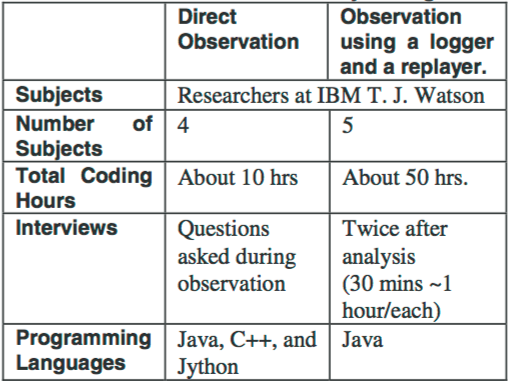
\includegraphics[width=7cm]{ooplStudy}
\caption{Description of IBM Study Environment}
\label{fig:oopl}
\end{figure}

According to this IBM study, they observed that 74\% of all copy and paste instances copied text less than a single line. These cases would be simple copies like copying a variable name, a type name, or a method declaration, and in these cases the command was most likely used for the sake of saving typing time. Of the remaining copies, however, they found that these were instances of copying blocks of code. Specifically in these cases the use of the copy and paste command created code duplicates and were heavily reflected in the resulting structure of the code base~\cite{ooplCP}.

The reason these structural code duplicates are important, is because there is an entire field of research focused on the errors that occur because of code duplicates~\cite{devWorkHabits}. Even though according to the IBM study these types of artifacts are only created roughly 25\% of the time, if you multiply that by the average 16 copy and paste instances per hour that means that the average professional programmer creates four non-trivial copy and paste dependencies per hour~\cite{ooplCP}. 

But what exactly do these non-trivial dependencies look like? To answer this we turn to a Microsoft study which consisted of thoroughly surveying and interviewing professional programmers who worked at Microsoft Corporation. This study is quite influential and has been cited 367 times since 2006, for the most part though it's influence is felt in other areas programmer habit study, though they specifically spent a section of their report discussing copy and paste habits. They conducted their study by creating a participant pool of 6000 programmers at Microsoft Corporation, and sending out two different surveys to subsets of size 200 from the participant pool. In both cases the subsets were asked roughly 200 questions and participation was nearly complete. Finally, after conducting both surveys, 11 individual programmers were individually interviewed~\cite{devWorkHabits}. 

In the results of their interviews these researches found that could create a taxonomy of categories of code duplication, and further detail the frequency of each category and importance of the problem~\cite{devWorkHabits}. Some of these categories are unrelated to our concerns on copy and paste habits, yet three are particularly relevant.

The first involves `example clones' which refers to code that is copied from an outside source and is used as an example, or a template, for use in a new context. These clones were actually the most studied, and the researchers found that it is difficult to say one way or another if the clones would be better off factored into a new abstraction. 

The second category is `scattered clones', or logical clones, and these are similar to the majority of copy and paste instances discussed earlier. For the most part these clones are simply the copy and paste of variable names, method headers, etc., and due to their nature they tend to propagate themselves throughout a code base. Because of this duplicitous nature, these clones can be hard to manage en masse, and multiple interviewees reported that when dealing with changing a root duplicate in these cases they would often ``hope for the best'' and rely on testers to find any  necessary changes.

Finally, the third relevant category for copy and pasting deals with `fork clones'. These types of clones occur when a developer `forks' another code base by literally copying the entire source to start new development on. In the production environment this can occur when a team needs to use code that another team isn't ready to ship, so they are forced to create a full copy of it and start tailoring it to their needs. In nearly every interview, the subjects reported that when possible it is best to avoid these types of clones, unless the only alternative is to implement the functionality from scratch. When these are necessary, a higher maintenance burden is placed on the new code base, and testing must be thorough~\cite{devWorkHabits}.

Clearly, the copy and paste command is incredibly influential in a programmer's work-flow, and while sometimes it can aid in creating non-trivial code clones, for the most part the negative effect of these clones is ambiguous. 

\section{Copy and Paste in Practice}\label{sec:copy}

All operating systems come with a system clipboard. It involves storing a single item, whether a piece of text, URL, image, or file to a place in memory. This item can then be retrieved multiple times and copied to appropriate locations. The main drawback of such a system is that when a new item is copied to memory, all information regarding the previous one is lost. If users wanted to obtain this information a second time, they would have to find the item and copy or cut it again~\cite{codeReuse}. See section~\ref{sec:patterns} for more information on why programmers typically use the copy and paste command.

There are many solutions that exist that make the system clipboard easier and quicker to use. \textit{X Window}~\cite{overlapWindow} is an application that speeds up interaction by having users drag to select text and then use the middle-click of the mouse to paste, instead of the default keyboard options. While this does offer more convenience, by saving some time, it doesn't address the main pain point with the system clipboard.

A significant improvement over this is the multi-item clipboard~\cite{cpHabits}. It stores multiple items in memory, and provides a way of retrieving them through shortcuts or a visual interface. The main advantage of this method is the time users save, as they don't have to go back to the source of an older item in order to paste it. Figure \ref{fig:Multi}~\cite{cpHabits} shows how there are fewer changes in window focus, thereby saving the user time. The study conducted by Stolee et al. monitored 15 users and recorded their copy-paste actions. In total, 2544 clipboard interactions were captured and the most frequent type of copy-paste actions was across windows, occurring 38\% of the time. They also observed that 20\% of the items on the clipboard were pasted multiple times, with the average number of destinations being three. In these situations, having a multi-item clipboard would significantly reduce the time taken to paste items previously copied, by allowing the user to paste without having to switch windows repeatedly.

These type of multi-item clipboards can be especially useful for programmers as shown by the IBM study discussed in section~\ref{sec:patterns} where researchers found that the average programmer copy and pastes code 16 times for every hour of programming~\cite{ooplCP}. A problem with these existing mutli-item solutions is that they are not targeted specifically at programmers. A clipboard manager targeted to programmers could help eliminate some of the common problems a programmer faces, many of which are discussed in detail in section~\ref{sec:features}.

An example of an already existing multi-item clipboard plug-in for Eclipse, an IDE used primarily for Java development, is \textit{More Clipboard}~\cite{moreclipboard}. It keeps track of items copied and pasted and makes them available in a list that allows users to paste information several copies back. While this is useful, it fails at assisting programmers with other commonly faced issues such as identifying the context, and detecting code cloning and design patterns. It also doesn't work too well with displaying large chunks of code, something we're looking to address in our proposed plug-in discussed in section~\ref{sec:conclusion}.

\section{Code Cloning}\label{sec:clones}

Our analysis of copy and paste usage in the Eclipse IDE falls into the general area of code cloning. Many of the problems addressed in sections~\ref{sec:patterns} and~\ref{sec:copy} can be better solved by applying techniques in code clone detection, together with an improved clipboard manager. Therefore, a preliminary understanding of the concepts and techniques of code cloning will be of great help for both our current project and further work. 

The concept of code clones in software engineering is a kind of similarity. According to Ira Baxter, ``Clones are segments of code that are similar according to some definition of similarity''. And this kind of similarity can be based on either program texts or semantics~\cite{frontiers}. The similarity of program text can be defined in terms of text tokens, syntax or data and control dependencies, while the similarity of semantics is harder to define and is undecided yet~\cite{frontiers}. Based on program text similarity, code clones can be classified into three types: exact clone, which is an exact copy of consecutive code fragments without any modification; parameter-substituted clone, which is a copy of code fragments where only parameters like identifiers or literals are substituted; and structure-substituted clone, which is a copy of code fragments where parts of the structure are changed. The relation of these three types of cloning can be best illustrated with a syntax tree, where replacing a leaf generates a parameter-substituted clone and replacing a sub-tree leads to a structure-substituted clone. 

To efficiently manage clones of code, clone detection methods are needed. There are several comparison based clone detection methods that help us locate and track clones. The simplest one is text comparison, which compares program text textually. It can be applied to any kind of program, but is sensitive to changes in parameters or sub-structures. An alternative method is token comparison, which first turns a program into streams of tokens and then tries to find similar token sequences. However, the mere lexical analysis may lead to incomplete or syntactically incorrect code blocks. Therefore, instead of comparing text content directly, we can transfer text content into vectors and compare metric vectors in terms of Euclidean distance. While in practice, Euclidean distance may not best fit the content, we need to select one metric that is independent of program text, yet significant in distance and widely applicable to various situations. 

Last but not least, we can compare program dependency graphs. A program dependency graph is constructed from data and control dependencies within the code and thus is resilient to changes in parameters or substructures. A typical clone detection process is shown in Figure \ref{fig:detect}~\cite{towards_tool}.

\begin{figure}[h]
\centering
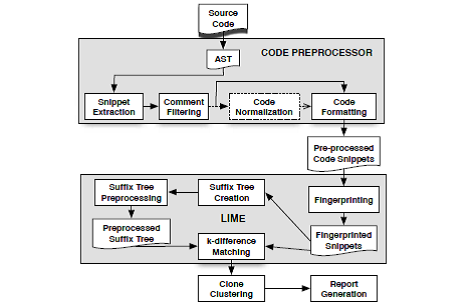
\includegraphics[width=10cm]{clone_detection}
\caption{Clone Detection Process}
\label{fig:detect}
\end{figure}

To understand the evolution of code clones, ~\cite{empirical} developed a model of clone genealogy. In this model, a code snippet with two attributes, text and location, is defined as the basic unit. The internal property Text can be compared to measure the similarity of two code snippets, while the external property Location is used to trace code snippets across multiple versions of program. Correspondingly, a \textit{TextSimilarity} function and a \textit{LocationOverlapping} function is defined respectively to measure the text similarity and location overlapping of two code snippets. Finally, several evolution patterns are defined to cover all possible changes to a code block. These patterns are self-expressed and can be organized into a directed acyclic graph to represent complex evolution patterns for further analysis. Figure \ref{fig:linea}~\cite{towards_tool} and Figure \ref{fig:genea}~\cite{towards_tool} are two examples of this model.

\begin{figure}[h]
\centering
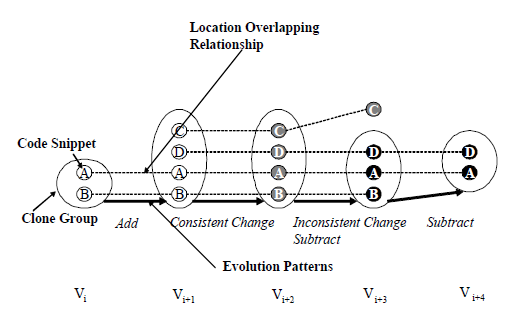
\includegraphics[width=8cm]{lineage}
\caption{An Example of Clone lineage}
\label{fig:linea}
\end{figure}

\begin{figure}[h]
\centering
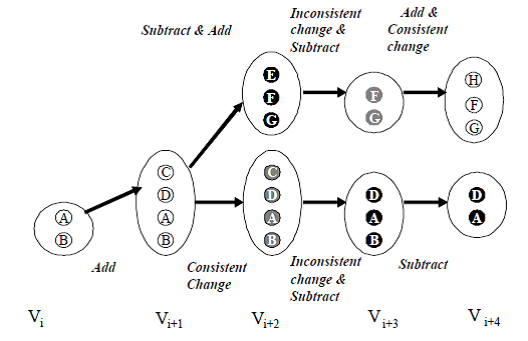
\includegraphics[width=7cm]{genealogy}
\caption{An Example of Clone Genealogy}
\label{fig:genea}
\end{figure}

Code clones are rooted in the limitation of programming languages, and are generated as programmers reuse pieces of code for strategies like forking, templating and customization. As long as programmers go on adopting strategies of forking to bootstrap development of similar solutions, or templating for abstraction and customization of new features, code clones will remain a big issue within software development~\cite{frontiers}. For this particular reason, understanding how clones evolve, examining the pros and cons of code clones, and furthermore detecting and managing clones in code will remain themes of software engineering. In addition, due to nature of the copy and paste command, code clones are inherently critical considerations when developing for the copy and paste habits of programmers.

\section{Project Goals}\label{sec:goals}

In this section, we focus on documenting some problem \textit{P}, with some user group \textit{U}, using some software tool \textit{T}, to achieve some goal \textit{G}, or \textit{PUGT} for short. Specifically, for our proposed project \textit{PUGT} is defined in the following ways.

\textit{P}: The problem we will focus on is more efficient copying and pasting. See sections~\ref{sec:patterns} and~\ref{sec:copy} for more details on what we mean by efficient, and how and why the copy and paste command is currently used.\\
\textit{U}: The user group we will target is Java programmers.\\
\textit{G}: The goal of this project is to create a clipboard manager which will provide features to improve copying and pasting solutions and combat programming errors introduced by the traditional copy and paste command discussed in section~\ref{sec:patterns}. We will describe these features in detail in section~\ref{sec:features}.\\
\textit{T}: The tool we will use to implement our clipboard manger is the Eclipse IDE, specifically in the form of an extension for the IDE referred to as a plug-in.

\subsection{Project Features}\label{sec:features} 

\subsubsection{Multi-item Clipboard}\label{multiCopy}

As discussed in section~\ref{sec:copy}, programmers often switch back and forth between windows to copy and paste. If we can design a clipboard that holds multiple item at a time, it will reduce window switching. For example, if a programmer needs to copy a student's name, email address, and institution to a form in a different window, a multi-item clipboard manager can hold each item separately and paste it altogether at once. With a multi-item clipboard solution this situation would be solved in only one instance of window switching, instead of the three instances it would require with traditional copying and pasting.
 
As well, multiple items can also be copied from multiple windows. Figure \ref{fig:Multi} compares two different variations of multiple item copying and pasting between current copy and paste functionality and our proposed multi-item clipboard's functionality~\cite{cpHabits}. The upper portion demonstrates copying multiple items from a single source as in our example of copying the student's information, while The bottom portion depicts copying items from multiple windows to a destination.
 
\begin{figure}[h]
\centering
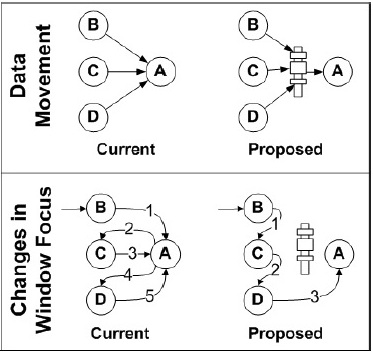
\includegraphics[width=6cm]{MultiItem}
\caption{Multiple Item Copy and Pasting}
\label{fig:Multi}
\end{figure} 

\subsubsection{System Wide copy}\label{systemCopy}
For this feature, we perform a greater analysis on the copy and paste operation, and consider when a programmer might copy information from outside the programming environment. As discussed in the Microsoft study in section~\ref{sec:patterns}, one of the frequent types of programmer copy and paste usages is when a programmer copies example code found outside of their current working environment, on the Internet for example~\cite{devWorkHabits}. In this case we would want our clipboard manager that is integrated into our programming environment to reflect this copy and display it with the rest of the copies that have been gathered from inside our IDE. A system wide copy feature simply extends on the functionality of our clipboard manager, by integrating it into the more global system wide uses of the copy and paste command.

\subsubsection{Context Awareness}\label{context}
If we assume the inclusion of the multi-item feature into our clipboard manager we are presented with an additional challenge, how do we present these items? This problem itself can be broken down into two large categories, how do we display these items individually, and how do we order them contextually? A context awareness feature of our clipboard manager answers the latter of these two questions, while subsection~\ref{display} addresses the former. We can say our clipboard is context aware if it is able to effectively display each item in our clipboard in a meaningful order, and if it has the ability to sort these in multiple ways other than the default reverse chronological.
    
For example, some clipboard managers like \textit{Citrine}~\cite{Citrine} and \textit{Entity Quick Click}~\cite{Entity} partially support context awareness features. \textit{Citrine} describes itself as an intelligent clipboard: it copies data, extracts contextual information and partitions the data accordingly. Because of this partitioning it is able to order the items in different manners. \textit{Entity Quick Click} orders its items in a similar fashion as \textit{Citrine}, by gathering contextual information, and partitioning the data accordingly.

\subsubsection{Intelligent Display Manager}\label{display}
As discussed in subsection~\ref{context} an important feature of a clipboard manager revolves around how we effectively display the copied items from our clipboard. To illustrate this feature we look at a smart clipboard manager for Windows called \textit{Kana Clip}~\cite{KanaClip}. This program is able to automatically monitor and store system wide clipboard data into its memory. In order to access the text entries saved to the clipboard, users make use of a hotkey which then presents the user with all of their recently copied items. As well, a list with all available options for the user is automatically displayed in a popup panel. 

Another example of a smart clipboard manager is \textit{Clipboard History}, which is shown in Figure \ref{fig:Clip_History}~\cite{ClipHistory}. Here we can see that the left pane is the user's clipboard history detailing what the user has recently copied to the clipboard, while the right pane displays permanent clips known as `stickies', which can not be overwritten. This addition of a `stickies' is a great feature for things that the user knows they will need to access frequently in the future. Features demonstrated by programs like \textit{Kana Clip} and \textit{Clipboard History} will enhance our clipboard manager regarding ordering and displaying large chunks of code and allowing the user to designate certain copies as important for future use.

\begin{figure}[h]
\centering
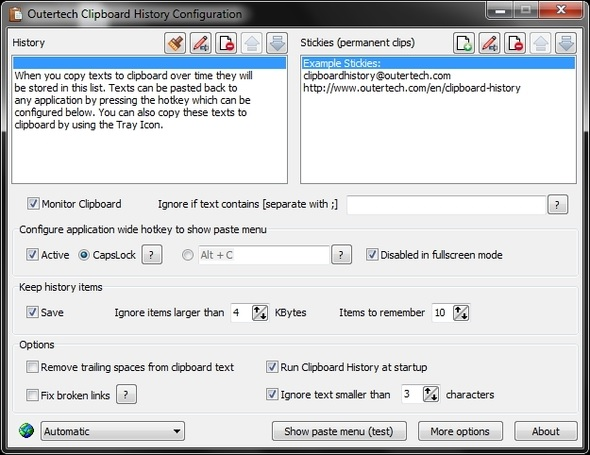
\includegraphics[width=8.5cm]{ClipHistory}
\caption{Screenshot of \textit{Clipboard History}}
\label{fig:Clip_History}
\end{figure} 

\subsubsection{Code Cloning}
As discussed in section~\ref{sec:clones}, when programmers copy and paste within their program environments frequently artifacts of code duplication, or code clones, will be generated. Code clones can be tricky to handle, and frequently a programmer might not even be aware that they have created them. Luckily, there are tools for code clone detection~\cite{CloneTag}, and these could be implemented into our clipboard manager as a feature. By integrating code clone detection and awareness into our manager we can directly alleviate one of the biggest problems related to programmers copying and pasting. As well, there are no examples of current clipboard managers that address this problem so it would be a novel contribution.

\subsubsection{Design Pattern Detection}
In software engineering design patterns are essential architectural tools that help development of software solutions. A feature of our clipboard manager could deal with detecting which design pattern the programmer is implementing and aiding them in managing it. Essentially, there are papers such as~\cite{Pattern} that discuss the state-of-the-art pattern detection tools which we could implement into our clipboard manager. By having a clipboard that uses the copy history to detect design patterns, our tool could detect when programmers are following recommended patterns or are straying off course, offering assistance as needed.

\subsubsection{Touch Screen Interactions}
With the onset of laptops and computer monitors integrating touch screen capabilities, there lies a great untapped potential of desktop software features which uniquely use touch as a modality of interaction. One feature of our clipboard manager could be to integrate touch controls into our plug-in, such that programmers can tap on code fragments to be copied, and paste at desired locations by dragging.

\section{Conclusion}\label{sec:conclusion}

All programmers make use of the copy and paste operation as part of their work-flow while programming. Specifically an IBM study has shown that the average programmer performs copy and paste actions 16 times per hour just by using the default system clipboard~\cite{ooplCP}. Using the default system clipboard can lead to a few unintended consequences such as code cloning and code duplication, and a general reduction in productivity by having to switch between files, projects, and windows while copy-pasting code multiple times. One solution to the default system clipboard are tools known as clipboard managers.

While there are several clipboard managers that deal with some of these problems, not many of them are targeted specifically at programmers, and the ones that are do not implement features to tackle all of these problems.

We propose \textit{Clipit}, an intelligent Eclipse IDE plug-in that is a clipboard manager extension designed specifically to improve a programmers productivity, and reduce programming errors commonly associated with copying and pasting. Of the features described in section~\ref{sec:features}, our implementation of \textit{Clipit} will provide features~\ref{multiCopy},~\ref{systemCopy},~\ref{context}, and~\ref{display}. Our resulting clipboard manager will be able to hold multiple items, manage copies made from outside the Eclipse IDE, display these items intelligently, and provide context awareness through smart ordering. \textit{Clipit} will also use standard keyboard shortcuts already familiar to programmers, making it easy to use.

\bibliographystyle{abbrv}
\bibliography{citations}

%\balancecolumns 

\end{document}